\documentclass[12pt]{report}
\title{\textbf{\Huge View Maintenance \\ in Data Warehousing } }
\author{CV Hariharan \bullet 1610110147 \\ Divya Raj \bullet 1610110123 \\ Devansh Purohit \bullet 1610110116}
\date{}

\usepackage[margin=1.4in]{geometry}
\usepackage{graphicx}
\usepackage{float}
\usepackage{amsmath}

\begin{document}
\maketitle
\section*{Acknowledgment}
We would like to thank Dr. Sonia Khetarpaul, our instructor for the Advance Database Management course this semester, for helping us with this project and the report. She taught us the concepts needed for this project and was available to us for help, whenever we needed it. Thank you.\\
\\We would also like to thank Hemant Jain and Anjana Gosain for their amazing paper titled "A Comprehensive Study of View Maintenance Approaches in 
Data Warehousing Evolution". It was a source of great help throughout this project. \\
\\Also, huge gratitude towards Abdulaziz S. Almazyad and Mohammad Khubeb Siddiqui for their paper titled "Incremental View Maintenance: An Algorithmic 
Approach". It gave us great insight into the incremental approach to view maintenance and inspired the final solution that we implemented.
\\\\Finally, we would like to thank Github user AntonioL for his repository -  "factorized-incremental-maintenance". It provided us a code wise basis for the project and helped us get started.
\\\\All the relevant links can be found at the end of this report in the Bibliography section.
\tableofcontents
\newpage
\renewcommand{\thesection}{\arabic{section}}
\section{Introduction}
A data warehouse mainly stores integrated information over data from 
many different remote data sources for query and analysis. The 
integrated information at the data warehouse is stored in the form of 
materialized views. Using these materialized views, user queries may be 
answered quickly and efficiently as the information may be directly 
available. These materialized views must be maintained in answer to 
actual relation updates in the different remote sources. \\
One of the issues 
related to materialized views is that whether they should be recomputed 
or they should be adapted incrementally after every change in the base 
relations. \\
View maintenance is the process of updating a materialized 
view in response to changes to the underlying data is called view 
maintenance. There are several algorithms developed by different 
authors to ease the problem of view maintenance for data warehouse 
systems. \\
In this report, we document the already existing approaches in the field, describe the approach that we took and also show our findings and conclusions.

\section{Related Work}
The plant is a system, and a system needs harmonical contributions of some components. These components in their actual form are discussed below one by one. The work-flow of a thermal power plant is in the following manner. Fuel (which has generally large particle size) is crushed down to smaller particle size. It is then combusted to generate heat. This heat is then transferred to running water which then turns to high pressure steam. Generally, gases from the boiler exhaust are at high temperature and if this heat is not utilized will lead to a large amount of losses resulting in reduced boiler efficiency. So generally this waste heat is recovered by heating either air required for combustion or preheat water before sending it into a boiler. Gases are then allowed to pass through a dust collector or a bag filter to arrest dust particles so as to prevent air pollution before sending it to the atmosphere through a chimney.
\begin{figure}[H]
\centering 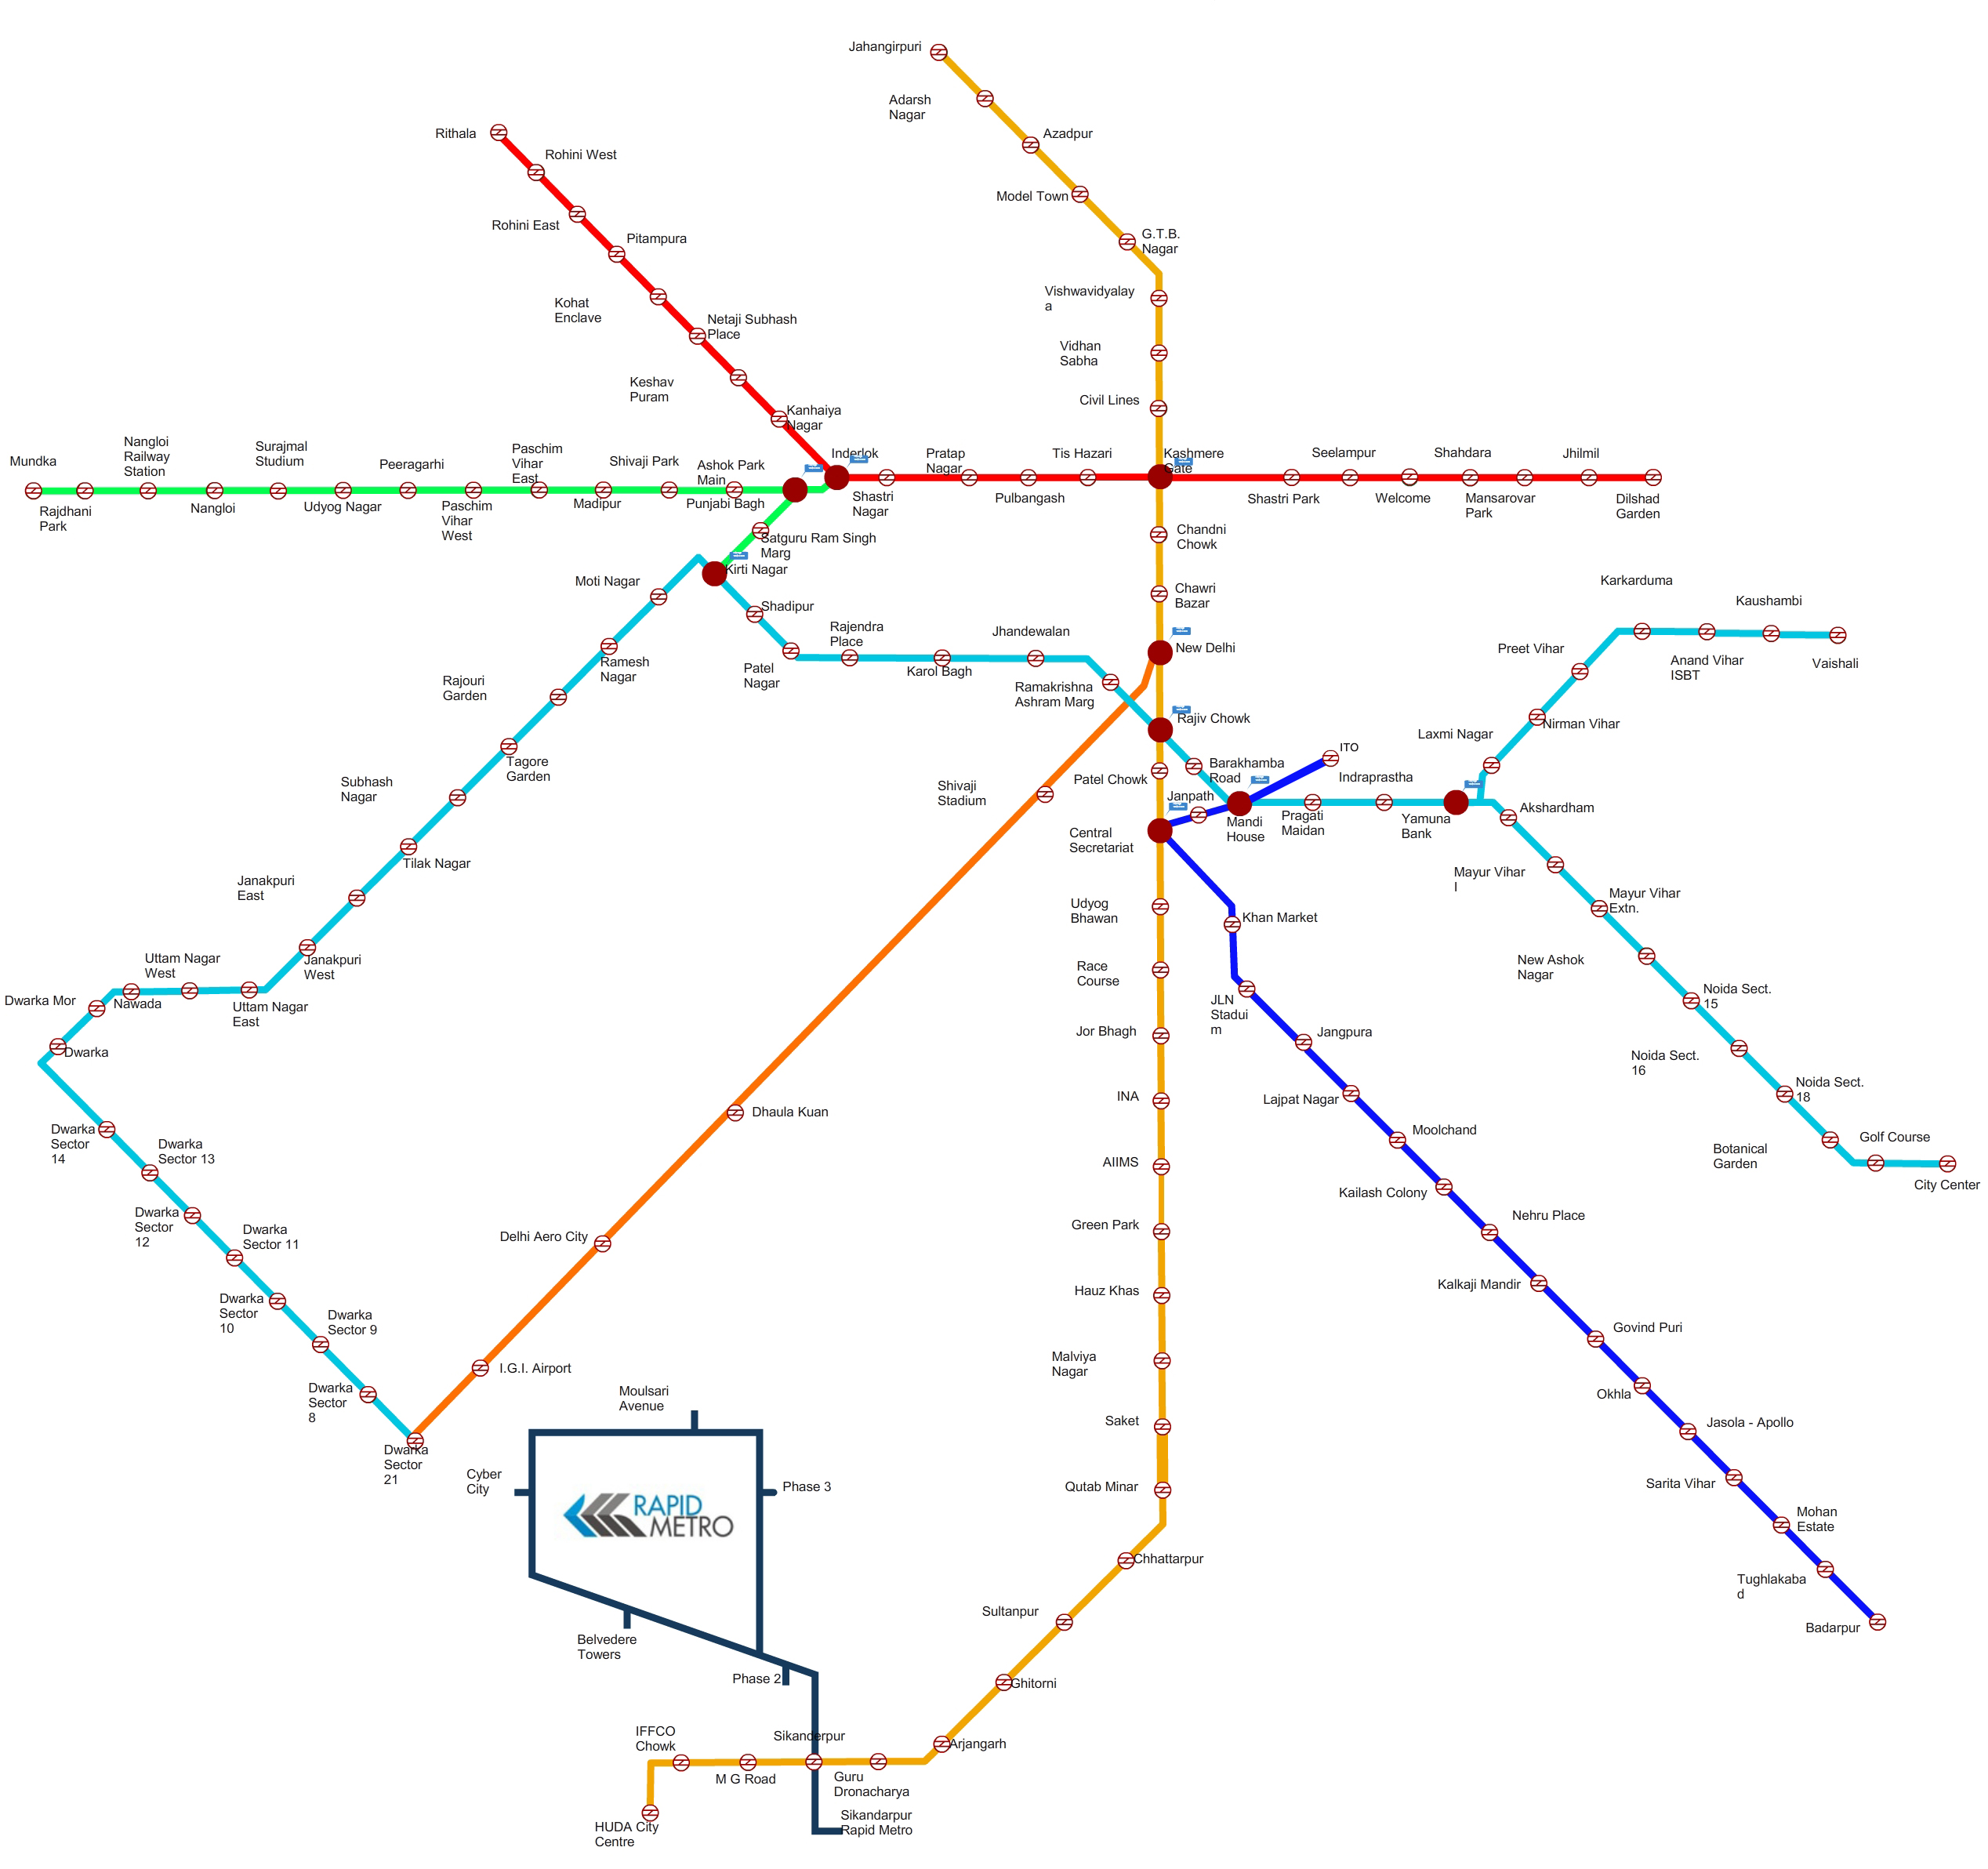
\includegraphics[width=0.9\textwidth]{images/pic1.jpg}
\caption{Image}
\end{figure}
\section{Proposed Approach}
Fuel is an important resource. Any plant which depends extensively on fuel needs to store it somewhere from where it could be used later on when the supply of fuel from the mine is improper. This is where a fuel storage facility comes into picture. \par In a thermal power plant, the first step in process of power generation is that the fuel is brought to breaker house with the help of belt conveyor, here light dust is separated with the help of rotary machine through the action of gravity. It further goes to the crusher where it is crushed to a size of about 50mm.
\section{Implementation and Results}
The water that has been converted to steam, is brought to the turbines under high pressure. This steam is used to rotate them. Normal water is taken from the river, and it contains a lot of dirt, suspended particulate matter (SPM), dissolved minerals and dissolved gases such as air etc. If the water fed to the boiler is not treated, it will reduce the life and efficiency of equipment by corroding the surfaces which may lead to overheating of pressure parts and explosions. \par This particulate matter is separated out by adding {\it alum} into the water. Alum coagulates the dirt and increases its density. Then, due to gravity, this coagulated matter settles down in the water which is then removed from it. 


\par After gravity separation, water softening is done by ion exchange process. As the hardness comes through the carbonates and bicarbonates of sodium and magnesium, these salts are removed from water anion exchange and cation exchange process. \par Water also contains dissolved oxygen and this leads to corrosion and fouling of boiler tubes and surfaces when it comes in their contact. So removing dissolved oxygen from water is done by adding oxygen scavengers and by using a Deaerator tank. Deaerator tank also acts as a feed water tank to store the feed water. On heating feed water in a deaerator tank decreases the solubility of air in water, thereby removing the dissolved air from the water.
\section{Conclusions and Limitations}
A boiler is a high pressure vessel used to generate high pressure steam at saturated temperatures. Water tube boiler consists of a furnace enclosed by the water tubes membrane. The crushed fuel from the crushers is fed into the boiler furnace over the grate. The hot air from the Forced Draft (FD) fan is mixed with the crushed fuel causing combustion of fuel.
Combustion of fuel generates a lot of radiation heat which is transferred to water in the membrane tubes. Flue gases generated during combustion travel at high velocity across the convection bank of tubes thereby heating water through convection heat transfer. Hot water is sent to a boiler drum at high pressure through the feed water pump. The boiler tubes which are in contact with low temperature acts as downcomers to circulate the water while the tubes which are in contact with high temperature acts as risers to carry steam. This leads to an effective circulation of water thereby preventing the tubes from getting overheated.

Steam leaving the boiler is at a saturated temperature and pressure but there are a lot of heat losses during its transportation to the turbines. So to increase the quality of steam, steam Superheater is installed in a radiative section of a boiler to increase its temperature and dryness fraction without increasing its pressure as well as to accommodate for the transportation temperature losses.

The exhaust gases leaving the boiler are generally at high temperature and this waste heat is extracted by installing an Economiser or Water Pre heaters to preheat the feed water to the boiler and Air Preheaters to pre-heat the air coming from the Forced Draft Fan required for the combustion of fuel. Installing this equipment help to decrease the flue gas temperature thereby increasing the efficiency.

The flue gases leaving the boiler also contain some ash particles, so to reduce the air pollution, flue gases are allowed to pass through the Dust Collectors and Bag Filters to remove the ash particulates from the flue gases and are sometimes passed through the Wet Scrubbers to decrease the sulfur content from the gases.

The flue gases are drawn through this equipment using an Induced Draft (ID) Fan which is designed for a fixed capacity and head to prevent any back pressure. After the ID fan, flue gases are exhausted off into the atmosphere using a chimney.
\\ 
\begin{thebibliography}{999}
\bibitem{lambport}
https://www.youtube.com/watch?v=8uwrMLrqQlU
\bibitem{lambport}
http://www.thermodyneboilers.com/components-working-thermal-power-plant/
\bibitem{lambport}
https://en.wikipedia.org/wiki/File:PowerStation2.svg
\end{thebibliography}
\end{document}